{[}\href{languages.html}{Previous: Non English language support}{]}
{[}\href{index.html}{Contents}{]} {[}\href{todo.html}{Next: Future
Features \& Known Issues}{]}

\section{Divergence From Randomness (DFR)
Framework}\label{divergence-from-randomness-dfr-framework}

The Divergence from Randomness (DFR) paradigm is a generalisation of one
of the very first models of Information Retrieval, Harter's 2-Poisson
indexing-model~{[}\protect\hyperlink{1}{1}{]}. The 2-Poisson model is
based on the hypothesis that the level of treatment of the informative
words is witnessed by an \emph{elite set} of documents, in which these
words occur to a relatively greater extent than in the rest of the
documents.

On the other hand, there are words, which do not possess elite
documents, and thus their frequency follows a random distribution, which
is the \emph{single} Poisson model. Harter's model was first explored as
a retrieval-model by Robertson, Van Rijsbergen and
Porter~{[}\protect\hyperlink{4}{4}{]}. Successively it was combined with
standard probabilistic model by Robertson and
Walker~{[}\protect\hyperlink{3}{3}{]} and gave birth to the family of
the BMs IR models (among them there is the well-known BM25 which is at
the basis the Okapi system).

DFR models are obtained by instantiating the three components of the
framework: \protect\hyperlink{randomnessmodel}{selecting a basic
randomness model}, \protect\hyperlink{firstnorm}{applying the first
normalisation} and \protect\hyperlink{freqnormalisation}{normalising the
term frequencies}.

\href{}{}

\subsection{Basic Randomness Models}\label{basic-randomness-models}

The DFR models are based on this simple idea: "The more the divergence
of the within-document term-frequency from its frequency within the
collection, the more the information carried by the word \emph{t} in the
document \emph{d}". In other words the term-weight is inversely related
to the probability of term-frequency within the document \emph{d}
obtained by a model \emph{M} of randomness:

\href{}{}

\begin{longtable}[]{@{}ll@{}}
\toprule
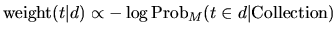
\includegraphics[width=3.53125in,height=0.35417in]{images/img1.png} &
(1)\tabularnewline
\bottomrule
\end{longtable}

where the subscript \emph{M} stands for the type of model of randomness
employed to compute the probability. In order to choose the appropriate
model \emph{M} of randomness, we can use different urn models. IR is
thus seen as a probabilistic process, which uses random drawings from
urn models, or equivalently random placement of coloured balls into
urns. Instead of \emph{urns} we have \emph{documents}, and instead of
different \emph{colours} we have different \emph{terms}, where each term
occurs with some multiplicity in the urns as anyone of a number of
related words or phrases which are called \emph{tokens} of that term.
There are many ways to choose \emph{M}, each of these provides a
\emph{basic DFR model}. The basic models are derived in the following
table.

Basic DFR Models

D

Divergence approximation of the binomial

\href{javadoc/org/terrier/matching/models/basicmodel/P.html}{P}

Approximation of the binomial

\href{javadoc/org/terrier/matching/models/basicmodel/B.html}{B\textsubscript{E}}

Bose-Einstein distribution

G

Geometric approximation of the Bose-Einstein

\href{javadoc/org/terrier/matching/models/basicmodel/In.html}{I(n)}

Inverse Document Frequency model

\href{javadoc/org/terrier/matching/models/basicmodel/IF.html}{I(F)}

Inverse Term Frequency model

\href{javadoc/org/terrier/matching/models/basicmodel/In_exp.html}{I(n\textsubscript{e})}

Inverse Expected Document Frequency model

If the model \emph{M} is the binomial distribution, then the basic model
is \emph{P} and computes the
value\protect\hyperlink{footnote1}{\textsuperscript{1}}:

\href{}{}

\begin{longtable}[]{@{}ll@{}}
\toprule
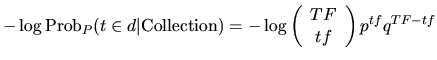
\includegraphics[width=4.55208in,height=0.62500in]{images/img2.png} &
(2)\tabularnewline
\bottomrule
\end{longtable}

where:

\begin{itemize}
\tightlist
\item
  \emph{TF} is the term-frequency of the term \emph{t} in the Collection
\item
  \emph{tf} is the term-frequency of the term \emph{t} in the document
  \emph{d}
\item
  \emph{N} is the number of documents in the Collection
\item
  \emph{p} is 1/\emph{N} and \emph{q}=1-\emph{p}
\end{itemize}

Similarly, if the model \emph{M} is the geometric distribution, then the
basic model is \emph{G} and computes the value:

\href{}{}

\begin{longtable}[]{@{}ll@{}}
\toprule
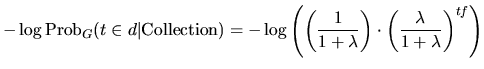
\includegraphics[width=5.04167in,height=0.71875in]{images/img11.png} &
(3)\tabularnewline
\bottomrule
\end{longtable}

where λ = \emph{F}/\emph{N}.

\href{}{}

\subsection{First Normalisation}\label{first-normalisation}

When a rare term does not occur in a document then it has almost zero
probability of being informative for the document. On the contrary, if a
rare term has many occurrences in a document then it has a very high
probability (almost the certainty) to be informative for the topic
described by the document. Similarly to Ponte and
Croft's~{[}\protect\hyperlink{2}{2}{]} language model, we include a risk
component in the DFR models. If the term-frequency in the document is
high then the risk for the term of not being informative is minimal. In
such a case Formula \protect\hyperlink{Formula:basic}{(1)} gives a high
value, but a \emph{minimal risk} has also the negative effect of
providing a \emph{small} information gain. Therefore, instead of using
the full weight provided by the Formula
\protect\hyperlink{Formula:basic}{(1)}, we \emph{tune} or \emph{smooth}
the weight of Formula \protect\hyperlink{Formula:basic}{(1)} by
considering only the portion of it which is the amount of information
gained with the term:

\href{}{}

\begin{longtable}[]{@{}ll@{}}
\toprule
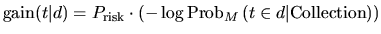
\includegraphics[width=3.96875in,height=0.35417in]{images/img14.png} &
(4)\tabularnewline
\bottomrule
\end{longtable}

The more the term occurs in the elite set, the less term-frequency is
due to randomness, and thus the smaller the probability
\emph{P\textsubscript{risk}} is, that is:

\href{}{}

\begin{longtable}[]{@{}ll@{}}
\toprule
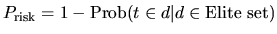
\includegraphics[width=2.88542in,height=0.35417in]{images/img16.png} &
(5)\tabularnewline
\bottomrule
\end{longtable}

We use two models for computing the information-gain with a term within
a document: the Laplace
\emph{\href{javadoc/org/terrier/matching/models/aftereffect/L.html}{L}}
model and the ratio of two Bernoulli's processes
\emph{\href{javadoc/org/terrier/matching/models/aftereffect/B.html}{B}}:

\href{}{}

\begin{longtable}[]{@{}ll@{}}
\toprule
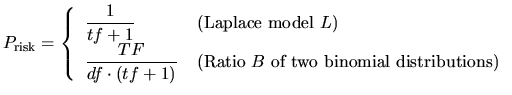
\includegraphics[width=5.33333in,height=0.98958in]{images/img19.png} &
(6)\tabularnewline
\bottomrule
\end{longtable}

where \emph{df} is the number of documents containing the term.

\href{}{}

\subsection{Term Frequency
Normalisation}\label{term-frequency-normalisation}

Before using Formula \protect\hyperlink{Formula:DFR}{(4)} the
document-length \emph{dl} is normalised to a standard length \emph{sl}.
Consequently, the term-frequencies \emph{tf} are also recomputed with
respect to the standard document-length, that is:

\href{}{}

\begin{longtable}[]{@{}ll@{}}
\toprule
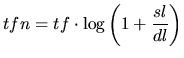
\includegraphics[width=1.91667in,height=0.60417in]{images/img23.png} &
(7)\tabularnewline
\bottomrule
\end{longtable}

A more flexible formula, referred to as
\emph{\href{javadoc/org/terrier/matching/models/normalisation/Normalisation2.html}{Normalisation2}},
is given below:

\href{}{}

\begin{longtable}[]{@{}ll@{}}
\toprule
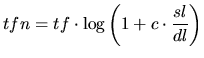
\includegraphics[width=2.12500in,height=0.60417in]{images/img24.png} &
(8)\tabularnewline
\bottomrule
\end{longtable}

\emph{DFR Models are finally obtained from the generating Formula
\protect\hyperlink{Formula:DFR}{(4)}, using a basic DFR model (such as
Formulae \protect\hyperlink{Formula:binomial}{(2)} or
\protect\hyperlink{Formula:geometric}{(3)}) in combination with a model
of information-gain (such as Formula
\protect\hyperlink{Formula:riskLB}{6}) and normalising the
term-frequency (such as in Formula \protect\hyperlink{Formula:tfn}{(7)}
or Formula \protect\hyperlink{Furmula:tfn2}{(8)}).}

\href{}{}

\subsection{DFR Models in Terrier}\label{dfr-models-in-terrier}

Included with Terrier, are many of the DFR models, including:

\begin{longtable}[]{@{}ll@{}}
\toprule
Model & Description\tabularnewline
BB2 & Bernoulli-Einstein model with Bernoulli after-effect and
normalisation 2.\tabularnewline
IFB2 & Inverse Term Frequency model with Bernoulli after-effect and
normalisation 2.\tabularnewline
In\_expB2 & Inverse Expected Document Frequency model with Bernoulli
after-effect and normalisation 2. The logarithms are base 2. This model
can be used for classic ad-hoc tasks.\tabularnewline
In\_expC2 & Inverse Expected Document Frequency model with Bernoulli
after-effect and normalisation 2. The logarithms are base e. This model
can be used for classic ad-hoc tasks.\tabularnewline
InL2 & Inverse Document Frequency model with Laplace after-effect and
normalisation 2. This model can be used for tasks that require early
precision.\tabularnewline
PL2 & Poisson model with Laplace after-effect and normalisation 2. This
model can be used for tasks that require early precision
{[}\protect\hyperlink{7}{7}, \protect\hyperlink{8}{8}{]}\tabularnewline
\bottomrule
\end{longtable}

Recommended settings for various collection are provided in
\href{trec_examples.html\#paramsettings}{Example TREC Experiments}.

Another provided
\href{javadoc/org/terrier/matching/models/DFR_BM25.html}{weighting
model} is a derivation of the BM25 formula from the Divergence From
Randomness framework. Finally, Terrier also provides a
\href{javadoc/org/terrier/matching/models/DFRWeightingModel.html}{generic
DFR weighting model}, which allows any DFR model to be
\href{extend_retrieval.html}{generated and evaluated}.

\href{}{}

\subsection{Query Expansion}\label{query-expansion}

The query expansion mechanism extracts the most informative terms from
the top-returned documents as the expanded query terms. In this
expansion process, terms in the top-returned documents are weighted
using a particular DFR term weighting model. Currently, Terrier deploys
the Bo1 (Bose-Einstein 1), Bo2 (Bose-Einstein 2) and KL
(Kullback-Leibler) term weighting models. The DFR term weighting models
follow a parameter-free approach in default.

An alternative approach is Rocchio's query expansion mechanism. A user
can switch to the latter approach by setting
\texttt{parameter.free.expansion} to \texttt{false} in the
\texttt{terrier.properties} file. The default value of the parameter
beta of Rocchio's approach is \texttt{0.4}. To change this parameter,
the user needs to specify the property rocchio\_beta in the
\texttt{terrier.properties} file.

\subsection{Fields}\label{fields}

DFR can encapsulate the importance of term occurrences occurring in
different fields in a variety of different ways:

\begin{enumerate}
\tightlist
\item
  Per-field normalisation: The frequencies from the different fields in
  the documents are normalised with respect to the statistics of lengths
  typical for that field. This is as performed by the
  \href{javadoc/org/terrier/matching/models/PL2F.html}{PL2F} weighting
  model. Other per-field normalisation models can be generated using the
  generic
  \href{javadoc/org/terrier/matching/models/PerFieldNormWeightingModel.html}{PerFieldNormWeightingModel}
  model.
\item
  Multinomial: The frequencies from the different fields are modelled in
  their divergence from the randomness expected by the term's
  occurrences in that field. The
  \href{javadoc/org/terrier/matching/models/ML2.html}{ML2} and
  \href{javadoc/org/terrier/matching/models/MDL2.html}{MDL2} models
  implement this weighting.
\end{enumerate}

\subsection{Proximity}\label{proximity}

Proximity can be handled within DFR, by considering the number of
occurrences of a pair of query terms within a window of pre-defined
size. In particular, the
\href{javadoc/org/terrier/matching/dsms/DFRDependenceScoreModifier.html}{DFRDependenceScoreModifier}
DSM implements the pBiL and pBiL2 models, which measure the randomness
compared to the document's length, rather than the statistics of the
pair in the corpus.

\href{}{}

\subsection{DFR Models and
Cross-Entropy}\label{dfr-models-and-cross-entropy}

A different interpretation of the gain-risk generating Formula
\protect\hyperlink{Formula:DFR}{(4)} can be explained by the notion of
cross-entropy. Shannon's mathematical theory of communication in the
1940s~{[}\protect\hyperlink{5}{5}{]} established that the minimal
average code word length is about the value of the entropy of the
probabilities of the source words. This result is known under the name
of the \emph{Noiseless Coding Theorem}. The term \emph{noiseless} refers
at the assumption of the theorem that there is no possibility of errors
in transmitting words. Nevertheless, it may happen that different
sources about the same information are available. In general each source
produces a different coding. In such cases, we can make a comparison of
the two sources of evidence using the cross-entropy. The cross entropy
is minimised when the two pairs of observations return the same
probability density function, and in such a case cross-entropy coincides
with the Shannon's entropy.

We possess two tests of randomness: the first test is
\emph{P\textsubscript{risk}} and is relative to the term distribution
within its elite set, while the second \emph{Prob\textsubscript{M}} is
relative to the document with respect the entire collection. The first
distribution can be treated as a new source of the term distribution,
while the coding of the term with the term distribution within the
collection can be considered as the primary source. The definition of
the cross-entropy relation of these two probabilities distribution is:

\href{}{}

\begin{longtable}[]{@{}ll@{}}
\toprule
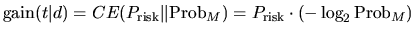
\includegraphics[width=4.31250in,height=0.35417in]{images/img26.png} &
(9)\tabularnewline
\bottomrule
\end{longtable}

Relation~\protect\hyperlink{Eq:cross-entropy:DFR}{(9)} is indeed
Relation~\protect\hyperlink{Formula:DFR}{(4)} of the DFR framework. DFR
models can be equivalently defined as the divergence of two
probabilities measuring the amount of randomness of two different
sources of evidence.

For more details about the Divergence from Randomness framework, you may
refer to the PhD thesis of Gianni Amati, or to Amati and Van
Rijsbergen's paper \emph{Probabilistic models of information retrieval
based on measuring divergence from randomness}, TOIS 20(4):357-389,
2002.

{[}\protect\hyperlink{1text}{1}{]} S.P. Harter. A probabilistic approach
to automatic keyword indexing. PhD thesis, Graduate Library, The
University of Chicago, Thesis No. T25146, 1974.\\
{[}\protect\hyperlink{2text}{2}{]} J. Ponte and B. Croft. A Language
Modeling Approach in Information Retrieval. In The 21st ACM SIGIR
Conference on Research and Development in Information Retrieval
(Melbourne, Australia, 1998), B. Croft, A.Moffat, and C.J. van
Rijsbergen, Eds., pp.275-281.\\
{[}\protect\hyperlink{3text}{3}{]} S.E. Robertson and S. Walker. Some
simple approximations to the 2-Poisson Model for Probabilistic Weighted
Retrieval. In Proceedings of the Seventeenth Annual International
ACM-SIGIR Conference on Research and Development in Information
Retrieval (Dublin, Ireland, June 1994), Springer-Verlag, pp. 232-241.\\
{[}\protect\hyperlink{4text}{4}{]} S.E. Robertson, C.J. van Risjbergen
and M. Porter. Probabilistic models of indexing and searching. In
Information retrieval Research, S.E. Robertson, C.J. van Risjbergen and
P. Williams, Eds. Butterworths, 1981, ch. 4, pp. 35-56.\\
{[}\protect\hyperlink{5text}{5}{]} C. Shannon and W. Weaver. The
Mathematical Theory of Communication. University of Illinois Press,
Urbana, Illinois, 1949.\\
{[}\protect\hyperlink{6text}{6}{]} B. He and I. Ounis. A study of
parameter tuning for term frequency normalization, in Proceedings of the
twelfth international conference on Information and knowledge
management, New Orleans, LA, USA, 2003.\\
{[}\protect\hyperlink{6text}{7}{]} B. He and I. Ounis. Term Frequency
Normalisation Tuning for BM25 and DFR Model, in Proceedings of the 27th
European Conference on Information Retrieval (ECIR'05), 2005.\\
{[}\protect\hyperlink{7text}{8}{]} V. Plachouras and I. Ounis.
Usefulness of Hyperlink Structure for Web Information Retrieval. In
Proceedings of ACM SIGIR 2004.\\
{[}\protect\hyperlink{8text}{9}{]} V. Plachouras, B. He and I. Ounis.
University of Glasgow in TREC 2004: experiments in Web, Robust and
Terabyte tracks with Terrier. In Proceedings of the 13th Text REtrieval
Conference (TREC 2004), 2004.

\subsection{Footnotes}\label{footnotes}

\href{}{}\textsuperscript{1}: We actually use approximating formulae for
the factorials. \protect\hyperlink{back1}{{[}back{]}}

{[}\href{languages.html}{Previous: Non English language support}{]}
{[}\href{index.html}{Contents}{]} {[}\href{todo.html}{Next: Future
Features \& Known Issues}{]}

\begin{center}\rule{0.5\linewidth}{\linethickness}\end{center}

Webpage: \url{http://terrier.org}\\
Contact:
\href{mailto:terrier@dcs.gla.ac.uk}{\nolinkurl{terrier@dcs.gla.ac.uk}}\\
\href{http://www.dcs.gla.ac.uk/}{School of Computing Science}\\
Copyright (C) 2004-2015 \href{http://www.gla.ac.uk/}{University of
Glasgow}. All Rights Reserved.\\
